% StudyOS Thesis-Finder — project presentation
% Build: latexmk -pdf studyos-thesis-finder.tex
\documentclass[11pt,aspectratio=169]{beamer}

\usetheme[progressbar=frametitle]{metropolis}
\usepackage[T1]{fontenc}
\usepackage[utf8]{inputenc}
\usepackage{booktabs}
\usepackage{tikz}
\usetikzlibrary{arrows.meta,positioning,shapes.misc}

% Slightly calmer metropolis accents
\definecolor{sosAccent}{HTML}{2A6F77}
\definecolor{sosDark}{HTML}{23373B}
\setbeamercolor{progress bar}{fg=sosAccent}
\setbeamercolor{frametitle}{bg=sosDark}
\setbeamercolor{alerted text}{fg=sosAccent}

\newcommand{\quotebox}[1]{%
  \begin{beamercolorbox}[rounded=true,sep=0.6em]{block body}%
    \itshape #1%
  \end{beamercolorbox}}

\title{StudyOS Thesis-Finder}
\subtitle{Minimal-maintenance discovery today; live candidate discovery tomorrow}
\author{StudyOS Team}
\institute{Department of Computer Science, University of Tübingen}
\date{July 2026}

\begin{document}

\maketitle

\begin{frame}{The problem, from both sides}
  \begin{columns}[T]
    \begin{column}{0.48\textwidth}
      \textbf{Students}
      \begin{itemize}
        \item Spend weeks figuring out which chairs even work on their interests
        \item See 4--5 listed topics, assume that is the whole lab, and never reach out
        \item Send generic cold emails to the wrong chairs
      \end{itemize}
    \end{column}
    \begin{column}{0.48\textwidth}
      \textbf{Professors}
      \begin{itemize}
        \item Receive far more inquiries than they can supervise \\ (one chair: 50+ inquiries for 20 slots)
        \item Lose time on rejection emails for mismatched inquiries
        \item Get low-signal first contacts that miss the chair's actual research
      \end{itemize}
    \end{column}
  \end{columns}
  \vspace{1em}
  \begin{center}
    \alert{Students and professors both lose when the first contact is poorly matched.}
  \end{center}
\end{frame}

\begin{frame}{What 27 professors told us --- before we built anything}
  We interviewed 27 professors in the CS department. The verdict on a classic
  \emph{topic-listing platform} was blunt or reluctant:
  \begin{itemize}
    \item \textbf{$\sim$50\%} do not want a central platform --- either already
      overrun with applicants, or convinced topics must be
      \emph{co-created in conversation}, not browsed from a list
    \item \textbf{$\sim$35\%} would try a tool --- but only if zero-friction,
      with no reminder emails, and stable for years
    \item \textbf{$\sim$15\%} recruit through other channels entirely
  \end{itemize}
  \quotebox{``Profs never update the topics. We've had many attempts in the
  department already.''}

  A topic platform was tried here around 2022 and failed --- for
  \alert{incentive} reasons, not UI reasons.
\end{frame}

\begin{frame}{The plan we started with --- and why we abandoned it}
  \begin{columns}[T]
    \begin{column}{0.5\textwidth}
      \textbf{First attempt}\\[0.3em]
      A hosted web app --- FastAPI $\cdot$ Celery $\cdot$ Postgres+pgvector
      $\cdot$ React --- scraping professors and serving a match portal.
      \smallskip
      \begin{itemize}
        \item Covered \textbf{CS Tübingen only}, would have gone stale within months
        \item Assumed HiWis would keep a scraping pipeline alive ``forever'', but with low effort
        \item Still needed someone to maintain brittle scraped state
      \end{itemize}
    \end{column}
    \begin{column}{0.5\textwidth}
      \textbf{The pivot}\\[0.3em]
      \begin{center}
        \alert{\large A maintained database is the wrong asset.}
      \end{center}
      \smallskip
      The professors' own signal pointed the way: \emph{build for students,
      read what already exists, ask chairs for nothing.}
      \smallskip

      So instead of maintaining scraped state, we packaged \emph{the search process}:
      today with a small reviewable backbone, and next with runtime candidate discovery.
    \end{column}
  \end{columns}
\end{frame}

\begin{frame}{The idea: ship the method, not the data}
  \small
  \begin{center}
    \alert{Zero professor participation. Minimal maintained state. Live verification at runtime.}
  \end{center}
  \vspace{0.3em}
  \begin{columns}[T]
    \begin{column}{0.48\textwidth}
      \textbf{Setup}\\[0.3em]
      Copy-and-paste the skill folder into a standard AI agent. No account,
      custom app, or professor-facing admin workflow.

      \medskip
      The current backbone is a small bridge: inspectable anchors plus live checks,
      not a large database of stale rows.
    \end{column}
    \begin{column}{0.48\textwidth}
      \textbf{Student path}\\[0.3em]
      \begin{enumerate}
        \item \textbf{Formulate}: build a six-dimension profile
        \item \textbf{Discover}: find chairs, groups, and companies with evidence
        \item \textbf{Prepare}: draft a specific first contact
      \end{enumerate}
      \medskip
      Deliverable: a \alert{map of the possibilities} --- what exists, why it fits,
      and where to start.
    \end{column}
  \end{columns}
\end{frame}

\begin{frame}{How it works: one flow, specialized skills}
  \centering
  \vspace{0.7em}
  \resizebox{0.96\textwidth}{!}{%
  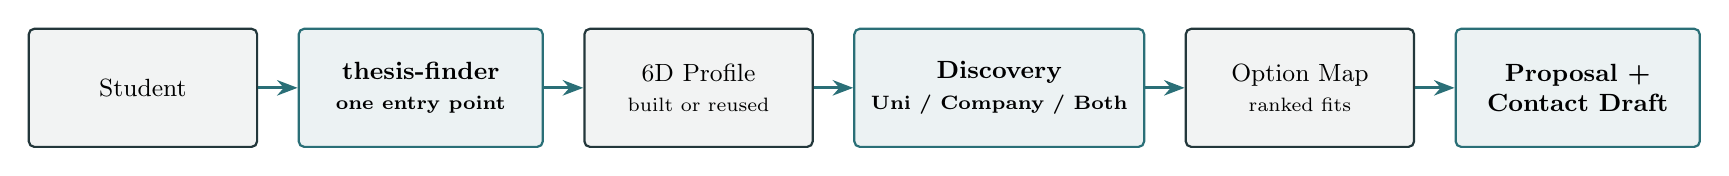
\begin{tikzpicture}[
      node distance=5mm,
      phase/.style={draw=sosDark, thick, rounded corners=2pt, fill=sosDark!6,
        align=center, font=\small, inner sep=6pt, minimum width=29mm, minimum height=15mm},
      skill/.style={draw=sosAccent, thick, rounded corners=2pt, fill=sosAccent!9,
        align=center, font=\small\bfseries, inner sep=6pt, minimum width=31mm, minimum height=15mm},
      arr/.style={-{Stealth[length=2.6mm]}, very thick, sosAccent}]
    \node[phase] (student) {Student};
    \node[skill, right=of student] (tf) {thesis-finder\\{\scriptsize one entry point}};
    \node[phase, right=of tf] (profile) {6D Profile\\{\scriptsize built or reused}};
    \node[skill, right=of profile] (discovery) {Discovery\\{\scriptsize Uni / Company / Both}};
    \node[phase, right=of discovery] (options) {Option Map\\{\scriptsize ranked fits}};
    \node[skill, right=of options] (contact) {Proposal +\\Contact Draft};

    \draw[arr] (student) -- (tf);
    \draw[arr] (tf) -- (profile);
    \draw[arr] (profile) -- (discovery);
    \draw[arr] (discovery) -- (options);
    \draw[arr] (options) -- (contact);
  \end{tikzpicture}}

  \vspace{1.2em}
  \small
  Discovery delegates to \alert{find-university-chairs} and/or
  \alert{find-company-thesis-options}. If needed, \alert{find-recent-papers}
  enriches the final proposal and contact draft.

  \vspace{0.7em}
  \scriptsize
  \textit{design-agent-skill is the meta-skill for redesigning or adding skills; it is not part of the student-facing path.}
\end{frame}

\begin{frame}{The core IP: a search method, not a store}
  \begin{columns}[T]
    \begin{column}{0.46\textwidth}
      \begin{center}
      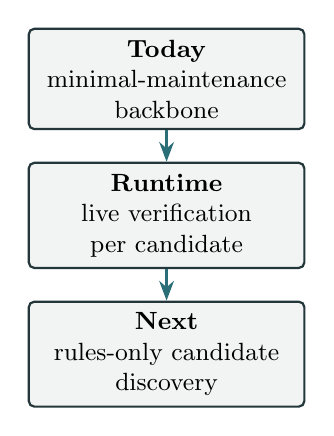
\begin{tikzpicture}[
          node distance=4mm,
          n/.style={draw=sosDark, thick, rounded corners=2pt, fill=sosDark!6,
            font=\small, inner sep=4pt, minimum width=35mm, align=center},
          arr/.style={-{Stealth[length=2.5mm]}, thick, sosAccent}]
        \node[n] (p) {\textbf{Today}\\minimal-maintenance\\backbone};
        \node[n, below=of p] (r) {\textbf{Runtime}\\live verification\\per candidate};
        \node[n, below=of r] (f) {\textbf{Next}\\rules-only candidate\\discovery};
        \draw[arr] (p) -- (r);
        \draw[arr] (r) -- (f);
      \end{tikzpicture}
      \end{center}
    \end{column}
    \begin{column}{0.52\textwidth}
      \footnotesize
      The current system is not a classic database, but it is not completely
      data-free either:
      \begin{itemize}
        \item \textbf{Small backbone} --- a reviewable set of structural anchors
          for faculties and BW companies
        \item \textbf{Search strategy} --- profile-to-query mappings, quality
          filters, dedup, and routing rules
        \item \textbf{Live verification} --- URLs, people, thesis signals, and
          evidence are checked during the run
      \end{itemize}
      The next version should replace stored anchors with \alert{rules-only
      candidate discovery} across multiple source axes.
    \end{column}
  \end{columns}
\end{frame}

\begin{frame}{Why not a maintained database}
  \renewcommand{\arraystretch}{1.22}
  \small
  \begin{center}
  \begin{tabular}{@{}p{0.30\textwidth}p{0.30\textwidth}p{0.30\textwidth}@{}}
    \toprule
    \textbf{Classic database} & \textbf{Current backbone} & \textbf{Future discovery} \\
    \midrule
    High maintenance & Minimal maintenance & Rules, not stored entities \\
    Full of stale rows & Small reviewable anchors & Fresh candidates per profile \\
    Needs backend/admin & Plain Markdown & Live search + verification \\
    Hard to port & Portable skill package & Portable when search tools exist \\
    \bottomrule
  \end{tabular}
  \end{center}
  \vspace{0.8em}
  \begin{center}
    \alert{The honest claim is not ``no data''. It is: keep durable knowledge in the method, and verify volatile facts live.}
  \end{center}
\end{frame}

\begin{frame}{Privacy and governance}
  \begin{itemize}
    \item \textbf{Student data never leaves the session.} The profile
      (interests, coursework, constraints) exists only in the student's own
      agent conversation --- nothing is stored or transmitted by us.
    \item \textbf{Only public academic data is used}: names, roles, research
      areas, and publications as published by chairs themselves ---
      GDPR-conscious by design.
    \item \textbf{Everything is inspectable.} Skills and references are plain
      text in a public repository; therefore easily adaptable by hand or AI agent.
    \item \textbf{No fabricated numbers.} A hard project rule: no placeholder
      metrics, no invented team sizes or citation counts.
  \end{itemize}
\end{frame}

\begin{frame}{Where we are, and what comes next}
  \small
  \begin{columns}[T]
    \begin{column}{0.31\textwidth}
      \textbf{Behind us}
      \begin{itemize}
        \item Interviewed 27 professors
        \item Dropped the full-stack app
        \item Shipped the skill-based tool
        \item Got some feedback by students.
      \end{itemize}
    \end{column}
    \begin{column}{0.33\textwidth}
      \textbf{Right now}
      \begin{itemize}
        \item Minimal-maintenance backbone as bridge
        \item Small, inspectable anchors
        \item Live verification during runs
      \end{itemize}
    \end{column}
    \begin{column}{0.33\textwidth}
      \textbf{Next}
      \begin{itemize}
        \item Dedicated candidate-discovery skills
        \item Rules for where and how to search
        \item Compare via command simulations
        \item upload to the big providers skill repositories
      \end{itemize}
    \end{column}
  \end{columns}
  \vspace{1.2em}
  \begin{center}
    \alert{Backbone today means pragmatic anchors; backbone tomorrow means discovery rules or alternatively some kind of automatic maintenance.}
  \end{center}
\end{frame}

\begin{frame}{TL;DR for professors}
  \begin{enumerate}
    \item \textbf{Nothing, by default.} The tool works from public pages
      and publications as they are.
    \item \textbf{Optionally:} a few research-area keywords, or a plain
      ``looking for / not looking for'' note.
    \item \textbf{(Almost) no maintenance.} No scraping, no database, no admin workflow, if our idea of self-maintaining discovery is working.
  \end{enumerate}
  \vspace{0.6em}
  \begin{center}
    \alert{Students get better discovery. Professors get fewer but better inquiries.\\
    Nobody is forced into a professor-facing admin workflow.}
  \end{center}
\end{frame}

\begin{frame}[standout]
  Thank you --- questions?
\end{frame}

\end{document}